\documentclass[tikz,border=6pt]{standalone}
\usepackage{amsmath,amssymb,mathtools,physics,bm,nicefrac,wasysym}
\usepackage{xcolor}

\definecolor{colone}{RGB}{180,60,60}
\definecolor{coltwo}{RGB}{60,110,180}
\definecolor{colthree}{RGB}{60,140,80}

\definecolor{accent}{HTML}{A13D2C}
\definecolor{accent2}{HTML}{2B5F6B}
\definecolor{muted}{HTML}{5A564F}
\definecolor{panel}{HTML}{F8F6F0}
\definecolor{linecol}{HTML}{D8D2C4}
\definecolor{ink}{HTML}{1E1C1A}
\definecolor{astroblue}{HTML}{1B4F72}
\definecolor{astrodark}{HTML}{17202A}
\definecolor{sunyellow}{HTML}{E8A33D}

\usetikzlibrary{calc,arrows.meta,positioning,decorations.pathreplacing,decorations.markings,angles,quotes,shapes.geometric}
\usepackage{tikz-3dplot}

\newcommand{\vecr}{\vec r}
\newcommand{\vecL}{\vec L}
\newcommand{\vecA}{\vec A}
\newcommand{\vecf}{\vec f}
\newcommand{\vecF}{\vec F}
\newcommand{\vecp}{\vec p}
\newcommand{\avg}[1]{\left\langle #1\right\rangle}
\newcommand{\vecx}{\vec x}
\newcommand{\hatn}{\hat n}
\newcommand{\rhat}{\hat r}
\newcommand{\phihat}{\hat\phi}
\newcommand{\thetahat}{\hat\theta}
\newcommand{\note}[1]{\textcolor{blue!60!black}{\textit{[#1]}}}

% Astronomical acronyms
\newcommand{\LST}{\mathrm{LST}}
\newcommand{\GST}{\mathrm{GST}}
\newcommand{\GMST}{\mathrm{GMST}}
\newcommand{\GAST}{\mathrm{GAST}}
\newcommand{\LMST}{\mathrm{LMST}}
\newcommand{\LAST}{\mathrm{LAST}}
\newcommand{\UT}{\mathrm{UT}}
\newcommand{\UTC}{\mathrm{UTC}}
\newcommand{\TAI}{\mathrm{TAI}}
\newcommand{\TT}{\mathrm{TT}}
\newcommand{\TDB}{\mathrm{TDB}}
\newcommand{\JD}{\mathrm{JD}}
\newcommand{\MJD}{\mathrm{MJD}}
\newcommand{\EoT}{\mathrm{EoT}}
\newcommand{\SNR}{\mathrm{SNR}}
\newcommand{\RON}{\mathrm{RON}}

% Helper commands for specific diagrams
\newcommand{\midlinelabel}[3]{
    \node (midlabel) at ($ (#1)!.5!(#2) $) {#3};
    \draw[stealth-] (#1) --  (midlabel);
    \draw[-stealth] (midlabel) -- (#2);
}
\newcommand{\midlinelabell}[3]{
    \node[fill = white, inner sep = 0.2pt, outer sep=3pt] (midlabel) at ($ (#1)!.5!(#2) $) {#3};
    \draw[stealth-] (#1) --  (midlabel);
    \draw[-stealth] (midlabel) -- (#2);
}
\newcommand{\midlinelabelll}[3]{
    \node[fill = white, inner sep = 0.2pt, outer sep=3pt,scale=0.6] (midlabel) at ($ (#1)!.5!(#2) $) {#3};
    \draw[stealth-] (#1) --  (midlabel);
    \draw[-stealth] (midlabel) -- (#2);
}



\begin{document}
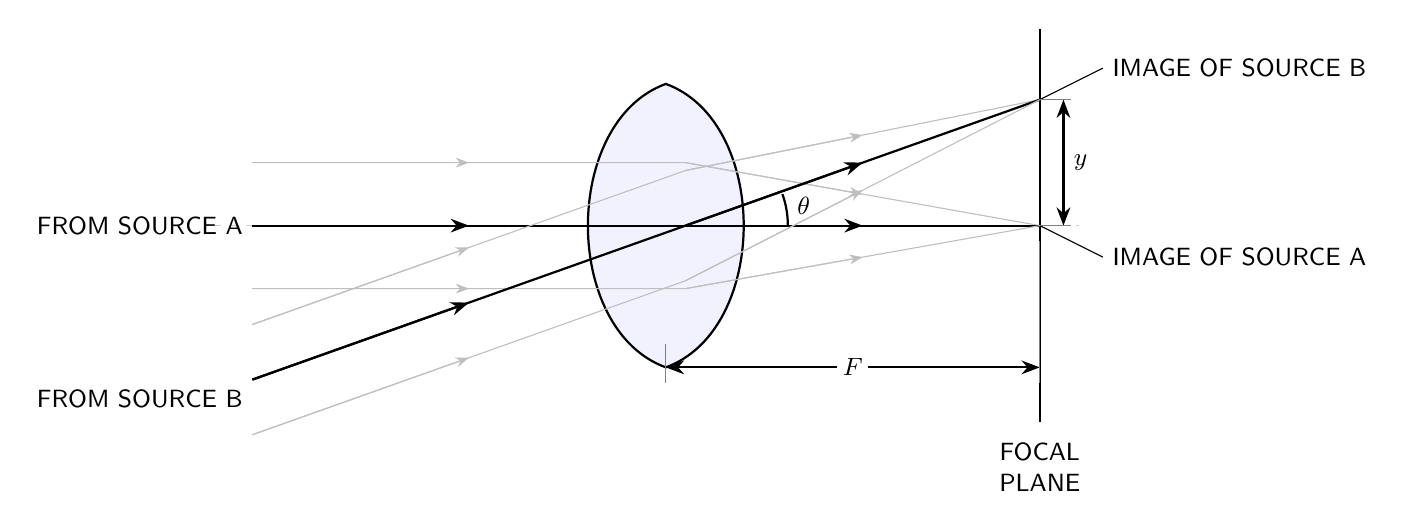
\begin{tikzpicture}[
        >=Stealth,
        font=\sffamily\small,
        ray/.style={thick, color=black},
        marginal/.style={thin, color=black!25} % Faded style for marginal/off-axis non-chief rays
    ]

        % Coordinates & Parameters
        \coordinate (LensCenter) at (0,0);
        \def\FocalLength{4.5}
        \def\ImageOffset{1.6} % Height y of off-axis image B
        
        \coordinate (ImageA) at (\FocalLength, 0);            % Center focal point (Image A)
        \coordinate (ImageB) at (\FocalLength, \ImageOffset);   % Off-axis focal point (Image B)
        
        % Focal Plane Line & Bottom Text
        \draw[thick] (\FocalLength, -2.5) -- (\FocalLength, 2.5);
        \node[below=4pt, align=center] at (\FocalLength, -2.5) {FOCAL\\PLANE};
        
        % Lens
        \draw[thick, fill=blue!5, draw=black] 
            (-0.25,-1.8) to[out=20, in=-20] (-0.25, 1.8) 
            to[out=-160, in=160] (-0.25,-1.8);

        % Optical Axis (Reference line)
        \draw[dashed, gray!40] (-6,0) -- (\FocalLength+0.5,0);

        % ================= SOURCE A (On-Axis: 3 Rays) =================
        % Ray A1 (Top horizontal ray - Faded)
        \draw[marginal] (-5.5, 0.8) -- (0, 0.8) -- (ImageA);
        \draw[marginal] (-5.5, 0.8) -- (-2.75, 0.8) [arrows={-Stealth}];
        \draw[marginal] (0, 0.8) -- ($(0,0.8)!0.5!(ImageA)$) [arrows={-Stealth}];

        % Ray A2 (Central optical axis ray / Chief Ray - Main Focus)
        \draw[ray] (-5.5, 0) -- (LensCenter) -- (ImageA);
        \draw[ray] (-5.5, 0) -- (-2.75, 0) [arrows={-Stealth}];
        \draw[ray] (LensCenter) -- ($0.5*(LensCenter)+0.5*(ImageA)$) [arrows={-Stealth}];

        % Ray A3 (Bottom horizontal ray - Faded)
        \draw[marginal] (-5.5, -0.8) -- (0, -0.8) -- (ImageA);
        \draw[marginal] (-5.5, -0.8) -- (-2.75, -0.8) [arrows={-Stealth}];
        \draw[marginal] (0, -0.8) -- ($(0,-0.8)!0.5!(ImageA)$) [arrows={-Stealth}];


        % ================= SOURCE B (Off-Axis: 3 Rays at Angle theta) =================
        % Ray B1 (Upper angled ray entering lens at y = 0.7 - Faded)
        \coordinate (B_start_top) at (-5.5, {0.7 - 5.5 * (\ImageOffset / \FocalLength)});
        \draw[marginal] (B_start_top) -- (0, 0.7) -- (ImageB);
        \draw[marginal] (B_start_top) -- ($0.5*(B_start_top)+0.5*(0,0.7)$) [arrows={-Stealth}];
        \draw[marginal] (0, 0.7) -- ($(0,0.7)!0.5!(ImageB)$) [arrows={-Stealth}];

        % Ray B2 (Central chief ray through lens center - Main Focus)
        \coordinate (B_start_chief) at (-5.5, {-5.5 * (\ImageOffset / \FocalLength)});
        \draw[ray] (B_start_chief) -- (LensCenter) -- (ImageB);
        \draw[ray] (B_start_chief) -- ($0.5*(B_start_chief)+0.5*(LensCenter)$) [arrows={-Stealth}];
        \draw[ray] (LensCenter) -- ($0.5*(LensCenter)+0.5*(ImageB)$) [arrows={-Stealth}];

        % Ray B3 (Lower angled ray entering lens at y = -0.7 - Faded)
        \coordinate (B_start_lower) at (-5.5, {-0.7 - 5.5 * (\ImageOffset / \FocalLength)});
        \draw[marginal] (B_start_lower) -- (0, -0.7) -- (ImageB);
        \draw[marginal] (B_start_lower) -- ($0.5*(B_start_lower)+0.5*(0,-0.7)$) [arrows={-Stealth}];
        \draw[marginal] (0, -0.7) -- ($(0,-0.7)!0.5!(ImageB)$) [arrows={-Stealth}];


        % ================= LABELS & MARKS =================
        % Angle theta mark
        \draw [thick] (1.3,0) arc (0:19.5:1.2);
        \node at (1.5, 0.25) {$\theta$};

        % Source & Image Labels
        \node[left] at (-5.5, 0) {FROM SOURCE A};
        \node[left] at (-5.5, -2.2) {FROM SOURCE B};

        \draw[thin] (ImageB) -- (\FocalLength+0.8, 2.0) node[right] {IMAGE OF SOURCE B};
        \draw[thin] (ImageA) -- (\FocalLength+0.8, -0.4) node[right] {IMAGE OF SOURCE A};

        % Dimension y (displacement on focal plane)
        \draw[<->, thick] (\FocalLength+0.3, 0) -- (\FocalLength+0.3, \ImageOffset) 
            node[midway, right] {$y$};
        \draw[thin, gray] (ImageA) -- (\FocalLength+0.4, 0);
        \draw[thin, gray] (ImageB) -- (\FocalLength+0.4, \ImageOffset);

        % Dimension F (focal length)
        \draw[<->, thick] (-0.25, -1.8) -- (\FocalLength, -1.8) 
            node[midway, fill=white, inner sep=2pt] {$F$};
        \draw[thin, gray] (-0.25, -1.5) -- (-0.25, -2.0);
        \draw[thin, gray] (\FocalLength, -0.2) -- (\FocalLength, -2.0);

    \end{tikzpicture}
\end{document}
